% Appendix A

\chapter{Diccionario Demogr\'afico} % Main appendix title

\label{AppendixA} % For referencing this appendix elsewhere, use \ref{AppendixA}

Sobre la base del trabajo de Roland Pressat en su \textit{``Diccionario de Demografía''} (Oikus-Tau Ediciones, 1987), los términos demográficos que recopilamos recogen las definiciones de los principales conceptos vistos en los cap\'itulos referentes a esta materia. Se ha intentado ser lo m\'as preciso posible en las definiciones para concretar al m\'aximo, pues cada t\'ermino da origen a otras entradas, no siendo el objeto de este ap\'endice servir de referencia en la materia, pues contiene un n\'umero limitado de entradas, sino servir de apoyo a la hora de definir términos y conceptos que no hayan quedado lo suficientemente claros en los capítulos anteriores.

\begin{multicols}{2}

\noindent\textbf{\huge{-- A --}}\\

\noindent \textbf{\Large{an\'alisis}}\\

\vspace{-0.3cm}
-- \textbf{\textit{demogr\'afico}}: forma de an\'alisis estad\'istico adaptado al estudio de las poblaciones humanas. Usando datos de diversas fuentes (censos, relaciones del Registro Civil y ocasionalmente datos o encuestas espec\'ificas), los transforma para terminar generando unas \textbf{tablas} (de mortalidad, de nupcialidad, de fecundidad, etc.) especificando las modalidades cuantitativas seg\'un las cuales las poblaciones se renuevan. El an\'alisis demogr\'afico suele distinguir entre \textbf{an\'alisis longitudinal} y \textbf{an\'alisis transversal}.\\

\vspace{-0.3cm}
-- \textbf{\textit{longitudinal}}: an\'alisis aplicado a las manifestaciones de un \textbf{fen\'omeno} en una \textbf{cohorte}. Se lleva a cabo partiendo de la construcci\'on de las tablas espec\'ificas del fen\'omeno considerado. Se utiliza junto al \textbf{an\'alisis transversal}\\

\vspace{-0.3cm}
-- \textbf{\textit{por cohorte}}: v\'ease \textbf{an\'alisis longitudinal}.\\

\vspace{-0.3cm}
-- \textbf{\textit{transversal}}: an\'alisis aplicado a las manifestaciones de un \textbf{fen\'omeno} durante un per\'iodo dado, generalmente el a\~no civil. Se efect\'ua recurriendo a las tablas del momento y a ciertos indicios espec\'ificos  como el \textbf{\'indice sint\'etico de los acontecimientos reducidos}.\\

\noindent \textbf{\Large{aglomeración urbana}}\\

\vspace{-0.3cm}
Conjunto de municipios sobre los que se extiende el territorio de una \textbf{aglomeración de población} a lo largo de varias circunscripciones administrativas, suele comprender una ciudad central y pueblos o ciudades satélite a los que ésta ha absorbido en su crecimiento.\\

\noindent\textbf{\huge{-- B --}}\\

\noindent \textbf{\Large{bruta, -o}}\\

\vspace{-0.3cm}
Cualificativo aplicado a las medidas vinculadas a un \textbf{fenómeno} considerado en estado puro, es decir, sin interferencias eventuales con fenómenos que modifiquen el original.\\

\noindent\textbf{\huge{-- C --}}\\

\noindent \textbf{\Large{censo}}\\

\vspace{-0.3cm}
-- \textbf{\textit{de la poblaci\'on}}: conjunto de operaciones que permiten conocer el efectivo de la poblaci\'on de un territorio en una fecha dada, con detalles referentes a la distribuci\'on de esa poblaci\'on por unidad administrativa y seg\'un una gama m\'as o menos extensa de caracter\'isticas.\\

\noindent \textbf{\Large{cohorte}}\\

\vspace{-0.3cm}
Conjunto de personas o de parejas que han vivido un mismo acontecimiento demogr\'afico durante un per\'iodo dado. Las cohortes constituyen el soporte del \textbf{an\'alisis longitudinal}. Se habla de \textit{generaciones} cuando se trata de cohortes de nacimientos.\\

\noindent \textbf{\Large{crecimiento}}\\

\vspace{-0.3cm}
-- \textbf{\textit{de la poblaci\'on}}: variaci\'on de los efectivos de una poblaci\'on durante un per\'iodo. Por crecimiento tambi\'en se entiende disminuci\'on y debe entenderse como la variaci\'on de la poblaci\'on entre dos fechas 1 y 2, es decir $P_{2}-P_{1}$, siendo la suma del \textbf{crecimiento natural} $(N-D)$ y de la \textbf{migraci\'on neta} $(I-E)$. $$P_{2}-P_{1}=(N-D)+(I-E)$$\\

\vspace{-0.9cm}
-- \textbf{\textit{natural}}: variaci\'on del efectivo de una poblaci\'on, durante un per\'iodo, como resultado del balance entre nacimientos y defunciones.\\

\noindent\textbf{\huge{-- D --}}\\

\noindent \textbf{\Large{defunción}}\\

\vspace{-0.3cm}
Muerte o fallecimiento de una persona.\\

\noindent \textbf{\Large{demograf\'ia}}\\

\vspace{-0.3cm}
-- \textbf{\textit{pura}}: estudio de las poblaciones humanas en relaci\'on con su renovaci\'on por medio de los nacimientos, de las defunciones y de los movimientos migratorios. Este estudio se dedica a analizar y describir el estado de las poblaciones, esto es, su efectivo y su composici\'on seg\'un diferentes criterios (edad, sexo, estado civil, localizaci\'on geogr\'afica, etc.) y en diferentes fases: mediante la recopilaci\'on de datos estad\'isticos a partir de los \textbf{censos} de poblaci\'on, los extractos del estado civil incluso encuestas espec\'ficas que recogen informaciones respecto a actitudes, comportamientos y opiniones. El an\'alisis cuantitativo de estos datos es lo que se llama \textbf{an\'alisis demogr\'afico} y los resultados obtenidos son confrontados con otras ciencias conectadas con la demograf\'ia (biolog\'ia, econom\'ia, historia, sociolog\'ia, etc.) con el fin de explicar el origen de los resultados, de los comportamientos observados y consecuentemente, establecer previsiones demogr\'aficas.\\

\vspace{-0.3cm}
-- \textbf{\textit{econ\'omica}}: establece las relaciones rec\'iprocas entre poblaci\'on y econom\'ia.\\

\vspace{-0.3cm}
-- \textbf{\textit{hist\'orica}}: estudia las poblaciones antiguas y sobre todo, de las que no se dispone de datos estad\'isticos en las formas modernas (estad\'isticas de poblaci\'on y censos).\\

\vspace{-0.3cm}
-- \textbf{\textit{matem\'atica}}: tiene por objeto presentar las magnitudes del an\'alisis demogr\'afico y de las relaciones existentes utilizando el lenguaje matem\'atico.\\

\vspace{-0.3cm}
-- \textbf{\textit{social}}: trata de las relaciones de los estados y de los movimientos de poblaci\'on con la vida de las sociedades.\\

\vspace{-0.3cm}
-- \textbf{\textit{cualitativa}}: estudio, a escala de las poblaciones, de las caracter\'isticas f\'isicas e intelectuales de las personas que las componen, y de los factores que determinan estas caracter\'isticas.\\

\vspace{-0.3cm}
-- \textbf{\textit{cuantitativa}}: conjunto de observaciones, an\'alisis y desarrollos te\'oricos que ponen en juego los diferentes aspectos num\'ericos de ls cuestiones de poblaci\'on.\\

\noindent \textbf{\Large{despoblación}}\\

\vspace{-0.3cm}
Disminución de la población de un territorio, causada esencialmente por un exceso de las defunciones sobre los nacimientos.\\

\noindent \textbf{\Large{despoblamiento}}\\

\vspace{-0.3cm}
Disminución de la población de un territorio causada, principalmente, por la \textbf{emigración}.\\

\noindent\textbf{\huge{-- E --}}\\

\noindent \textbf{\Large{emigraci\'on}}\\

\vspace{-0.3cm}
Para un territorio dado, el t\'ermino se refiere, tanto a la \textbf{migraci\'on} o salida de una persona desde este territorio hacia el exterior, como al fen\'omeno caracterizado por este acontecimiento.\\

\noindent \textbf{\Large{esperanza}}\\

\vspace{-0.3cm}
--  \textbf{\textit{de vida a la edad `x'}}: según una tabla de mortalidad, es el número medio de años que le quedan de vida a una persona que ha alcanzado la edad \textit{x}.\\

\vspace{-0.3cm}
--  \textbf{\textit{de vida al nacer}}: según una tabla de mortalidad, es el número medio de años de vida de una persona tomado en el nacimiento.\\

\noindent \textbf{\Large{estructura de población}}\\

\vspace{-0.3cm}
Composición de una población según diversas características específicamente demográficas (sexo, edad, estado matrimonial, etc.) o no (grado de instrucción, actividad económica, etc.) consideradas aisladamente o en asociación.\\

\noindent\textbf{\huge{-- F --}}\\

\noindent \textbf{\Large{fecundidad}}\\

\vspace{-0.3cm}
Referido al número de hijos que se tienen. El término fecundidad se identifica con la frecuencia de los nacimientos que tienen lugar dentro del subconjunto en edad de procrear.\\

\noindent \textbf{\Large{fenómeno}}\\

\vspace{-0.3cm}
En demografía, el término fenómeno hacer referencia a la llegada súbita de acontecimientos de una categoría dada. Por ejemplo, a los acontecimientos de defunciones, le corresponde el fenómeno \textbf{mortalidad}.\\

\noindent \textbf{\Large{fertilidad}}\\

\vspace{-0.3cm}
Término referido a la capacidad biológica de tener hijos, independientemente de si se han tenido antes o si se llegará a tenerlos algún día.\\

\noindent \textbf{\Large{función supervivencia}}\\

\vspace{-0.3cm}
Función \textit{S(x)} asociada a una tabla de mortalidad, definida para el conjunto continuo de los valores de la edad \textit{x} e identificándose a los valores de la serie de los supervivientes $S_{x}$ en las edades en que estos vienen dadas en la tabla considerada.\\

\noindent\textbf{\huge{-- G --}}\\

\noindent \textbf{\Large{generaci\'on}}\\

\vspace{-0.3cm}
\textbf{Cohorte} particular constitu\'ida por el conjunto de las personas nacidas durante un per\'iodo dado, generalmente el a\~no civil.\\

\noindent \textbf{\Large{Gompertz}}\\

\vspace{-0.3cm}
--  \textbf{\textit{fórmula de}}: fórmula propuesta en 1825 por el actuario inglés Gompertz, referente al cociente instantáneo de mortalidad, expresado como una función exponencial de la edad:$$q(x)=Ae^{kx}$$

%\noindent\textbf{\huge{h}}\\

\noindent\textbf{\huge{-- I --}}\\

\noindent \textbf{\Large{inmigraci\'on}}\\

\vspace{-0.3cm}
Para un territorio dado, el t\'ermino se refiere, tanto a la \textbf{migraci\'on} o entrada de una persona desde el exterior a este territorio, como al fen\'omeno caracterizado por este acontecimiento.\\

%\noindent\textbf{\huge{j}}\\

%\noindent\textbf{\huge{k}}\\

\noindent\textbf{\huge{-- L --}}\\

\noindent \textbf{\Large{Lexis, diagrama de}}\\

\vspace{-0.3cm}
Soporte gr\'afico que permite establecer la correspondencia entre unas fechas de observaci\'on y las antig\"uedades de cohortes en esas fechas. Atribu\'ido inicialmente al soci\'ologo y economista Wilhelm Lexis, tiene como base una red de paralelos con dos ejes rectangulares. En el eje horizontal se indican las fechas de observaci\'on y en el eje vertical, la duraciones de las cohortes (normalmente, la edad).

\hspace{-1cm}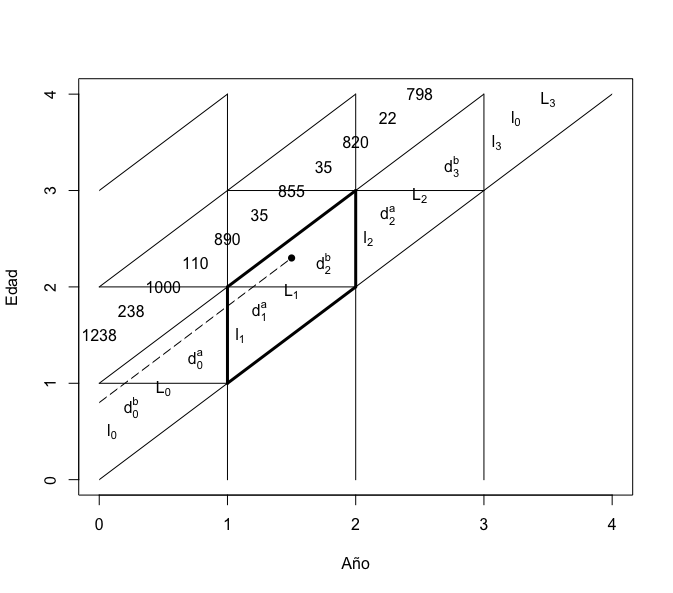
\includegraphics[scale=0.37]{Apendices/lexis.png}

Los pasillos determinados por dos l\'ineas diagonales consecutivas encierran todos los datos que afectan a una cohorte, seg\'un el sistema de convenciones que sigue.\\

\noindent \textbf{\Large{longevidad}}\\

\vspace{-0.3cm}
Concepto relacionado con la biolog\'ia, en el aspecto demogr\'afico, que es el que nos ocupa, es la extensi\'on m\'axima de la vida humana. Por extensi\'on, la palabra longevidad cuando se aplica a una generaci\'on o a una \'epoca da lugar a la expresi\'on \textit{longevidad media}, sin\'onimo de \textit{vida media} en esa generaci\'on o esa \'epoca.\\

\noindent\textbf{\huge{-- M --}}\\

\noindent \textbf{\Large{Makeham}}\\

\vspace{-0.3cm}
--  \textbf{\textit{fórmula de}}: fórmula propuesta en 1860 por el actuario inglés Makeham, referida al cociente instantáneo de mortalidad y que modifica la \textbf{fórmula de Gompertz}: $$q(x)=Ae^{kx}+k'.$$ Mediante la introducción del parámetro $k'$, Makeham pretendía tener en cuenta las muertes accidentales que se suman a las muertes por vejez, tomando la palabra accidental en un sentido amplio e incluyendo, por consiguiente, las defunciones de origen infeccioso.\\

\noindent \textbf{\Large{migraci\'on}}\\

\vspace{-0.3cm}
Desplazamiento de una persona motivado por un cambio de residencia. Tambi\'en se suele referir al fen\'omeno caracterizado por este tipo de acontecimiento. Dependiendo de la zona o territorio que consideremos, se definen otros conceptos, como los de \textbf{migraci\'on externa, migraci\'on interna, migraci\'on neta, migraci\'on total, emigraci\'on e inmigraci\'on.}\\

\vspace{-0.3cm}
-- \textbf{\textit{externa}}: migraci\'on entre dos lugares, uno situado dentro del territorio y el otro en el exterior. Normalmente se suele hablar de un pa\'is hacia otro y seg\'un el sentido se hablar\'a de \textbf{emigraci\'on} o de \textbf{inmigraci\'on}.\\

\vspace{-0.3cm}
-- \textbf{\textit{interna}}: migraci\'on entre dos lugares situados en el territorio.\\

\vspace{-0.3cm}
-- \textbf{\textit{neta}}: para un territorio y un período dados, es la diferencia entre la inmigración \textit{I} y la emigración \textit{E}.\\

\vspace{-0.3cm}
-- \textbf{\textit{total}}: para un territorio y un período dados, es la suma de las partidas y llegadas de emigrantes en ese territorio.\\

\noindent \textbf{\Large{migrante}}:\\

\vspace{-0.3cm}
persona que efectúa una \textbf{migración}\\

\noindent \textbf{\Large{mortalidad}}:\\

\vspace{-0.3cm}
-- \textbf{\textit{general}}: Fenómeno en relación con las defunciones. Suele hacer referencia implícita a la frecuencia del conjunto de las causas de defunciones en una población.\\

\vspace{-0.3cm}
-- \textbf{\textit{tablas de}}: instrumento de análisis demográfico cuyo fin es medir la incidencia de la mortalidad en la población que se estudia, con independencia de la estructura por edades de la misma, permitiendo analizar su evolución en el tiempo y en el espacio.\\

\noindent\textbf{\huge{-- N --}}\\

\noindent \textbf{\Large{natalidad}}\\

\vspace{-0.3cm}
Fenómeno relacionado con los nacimientos. Se suele tener en cuenta los nacimientos vivos, haciendo referencia, la palabra \texit{natalidad}, a la frecuencia de los nacimientos vivos en una población.\\

 \noindent \textbf{\Large{neta, -o}}\\
 
\vspace{-0.3cm}
Cualificativo aplicado a las medidas relacionadas con un fenómeno que tienen en cuenta las interferencias entre este fenómeno y fenómenos perturbadores, principalmente la fecundidad y la mortalidad.\\

%\noindent\textbf{\huge{o}}\\

\noindent\textbf{\huge{-- P --}}\\

\noindent \textbf{\Large{patrón}}\\

\vspace{-0.3cm}
-- \textbf{\textit{de fertilidad}}: distribución por edades de la fertilidad de las mujeres. La fertilidad está determinada ante todo, por la edad de las mujeres. La concepción solo puede comenzar después de la menarqu\'ia y no puede continuar, naturalmente, después de la menopausia.\\

\vspace{-0.3cm}
-- \textbf{\textit{de mortalidad}}: ver \textbf{tasa de mortalidad}.\\

\noindent \textbf{\Large{perspectiva demográfica}}\\

\vspace{-0.3cm}
Determinación de la evolución futura de una población establecida corrientemente sobre la base de hipótesis más o menos detalladas en cuanto al futuro de los componentes que rigen esa evolución. Estas hipótesis afectan por lo general a la fecundidad y a la mortalidad, y a veces a la nupcialidad.\\

\noindent \textbf{\Large{pir\'amide de edades}}\\

\vspace{-0.3cm}
Representación gráfica de la distribución por edad y sexo de la población. Gráficamente se representa mediante un doble histograma de frecuencias en el que en la derecha se refleja la población masculina y en la izquierda la población femenina.\\

\noindent \textbf{\Large{poblaci\'on}}\\

\vspace{-0.3cm}
Conjunto de individuos que coexisten en un \'area o espacio geogr\'afico determinado. El concepto de poblaci\'on no solamente es distinto para cada disciplina te\'orica, incluso para una misma disciplina dicho concepto admite muchas definiciones. En demograf\'ia la poblaci\'on puede ser entendida como objeto de an\'alisis estad\'istico o como mero volumen poblacional contabilizado en un determinado momento. De este modo, puede designar asimismo fracciones variadas de ese conjunto (poblaci\'on masculina y poblaci\'on femenina, poblaci\'on urbana y poblaci\'on rural, poblaci\'on activa, etc.) que no son sino \textit{subpoblaciones} con respecto a \'el.\\

\noindent \textbf{\Large{probabilidad de supervivencia}}\\

\vspace{-0.3cm}
Probabilidad, en la edad \textit{x}, de sobrevivir por lo menos hasta la edad $x+a$, que se anota $_{a}p_{x}$.\\

\noindent \textbf{\Large{proyección demográfica}}\\

\vspace{-0.3cm}
\textbf{Perspectiva demográfica} en la cual generalmente no existe la idea de previsión.\\


%\noindent\textbf{\huge{q}}\\

\noindent\textbf{\huge{-- R --}}\\

\noindent \textbf{\Large{renovación de la población}}\\

\vspace{-0.3cm}
Resultado del constante aporte de nuevos elementos en una población gracias a los nacimientos, y de la partida concomitante de elementos ancianos debida a las defunciones.\\

%\noindent\textbf{\huge{s}}\\

\noindent\textbf{\huge{-- T --}}\\

\noindent \textbf{\Large{tasa}}\\

\vspace{-0.3cm}
-- \textbf{\textit{bruta de mortalidad}}: número de defunciones persona-año registradas en una población. Se expresa en tantos por mil $$TBM=\frac{D^{t,t+1}}{0.5\times(P^{t}+P^{t+1})}\times 1000$$\\

\vspace{-0.5cm}
-- \textbf{\textit{de masculinidad}}: relaci\'on entre el efectivo masculino y el conjunto de una poblaci\'on.\\

\vspace{-0.3cm}
-- \textbf{\textit{de migraci\'on interna}}: para un territorio dado, relaci\'on entre el n\'umero de migraciones dentro del territorio durante un a\~no y la poblaci\'on media de ese a\~no, y m\'as generalmente, la relaci\'on entre el n\'umero de estas migraciones durante un per\'iodo y el n\'umero correspondiente de personas-a\~no durante el per\'iodo. En definitiva, no deja de ser la \textbf{tasa de movilidad interna} particular en la que intervienen las migraciones.\\

\vspace{-0.3cm}
-- \textbf{\textit{de migraci\'on neta}}: relaci\'on entre la \textbf{migraci\'on neta} de un a\~no y la poblaci\'on media de ese a\~no,  y m\'as generalmente, la relaci\'on entre la migraci\'on neta de un per\'iodo y el n\'umero correspondiente de personas-a\~no durante el per\'iodo. Se trata, asimismo de la diferencia entre la tasa de inmigraci\'on y la tasa de emigraci\'on.\\

\vspace{-0.3cm}
-- \textbf{\textit{de migraci\'on total}}: relaci\'on entre la \textbf{migraci\'on total} de un a\~no y la poblaci\'on media de ese a\~no,  y m\'as generalmente, la relaci\'on entre la migraci\'on total de un per\'iodo y el n\'umero correspondiente de personas-a\~no durante el per\'iodo.\\

\vspace{-0.3cm}
-- \textbf{\textit{de mortalidad}}: ver \textbf{\textit{tasa bruta de mortalidad}}.\\

\vspace{-0.3cm}
-- \textbf{\textit{infantil de mortalidad}}: defunciones ocurridas, estrictamente, durante el primer año de vida. Más allá de la edad exacta 1 se habla de \textit{mortalidad de la infancia}.\\

\vspace{-0.3cm}
-- \textbf{\textit{de feminidad}}: relaci\'on entre el efectivo femenino y el conjunto de una poblaci\'on.\\

\noindent \textbf{\Large{transición demográfica}}\\

\vspace{-0.3cm}
Se dice de la situación de una población cuya natalidad y mortalidad, o por lo menos uno de estos dos fenómenos, han dejado sus niveles tradicionales para dirigirse hacia los bajos niveles asociados a la fecundidad dirigida y al uso de los modernos métodos de lucha contra la mortalidad.\\

%\noindent\textbf{\huge{u}}\\

%\noindent\textbf{\huge{v}}\\

%\noindent\textbf{\huge{w}}\\

%\noindent\textbf{\huge{x}}\\

%\noindent\textbf{\huge{y}}\\

%\noindent\textbf{\huge{z}}\\
\end{multicols}